% article example for classicthesis.sty
\documentclass[12pt,a4paper]{article} % KOMA-Script article scrartcl
\usepackage{lipsum}
\usepackage{url}
\usepackage[nochapters]{classicthesis} % nochapters
%%%%%
\usepackage{geometry} % Required to change the page size to A4
\geometry{left=2cm,right=2cm,top=2.5cm,bottom=2.5cm}
\geometry{a4paper} % Set the page size to be A4 as opposed to the default US Letter
\usepackage{amssymb}

\usepackage{graphicx} % Required for including pictures
\usepackage{amsthm}
\usepackage{float} % Allows putting an [H] in \begin{figure} to specify the exact location of the figure
\usepackage{wrapfig} % Allows in-line images such as the example fish picture
\usepackage{amsmath}
\usepackage{hyperref}
\usepackage{listings}
\usepackage{color}
\usepackage{alltt}


\definecolor{dkgreen}{rgb}{0,0.6,0}
\definecolor{gray}{rgb}{0.5,0.5,0.5}
\definecolor{mauve}{rgb}{0.58,0,0.82}

\lstset{frame=tb,
	language=Verilog,
	aboveskip=3mm,
	belowskip=3mm,
	showstringspaces=false,
	columns=flexible,
	basicstyle={\small\ttfamily},
	numbers=none,
	numberstyle=\tiny\color{gray},
	keywordstyle=\color{blue},
	commentstyle=\color{dkgreen},
	stringstyle=\color{mauve},
	breaklines=true,
	breakatwhitespace=true,
	tabsize=3
}

% Theorem Styles
\newtheorem{theorem}{Theorem}[section]
\newtheorem{lemma}[theorem]{Lemma}
\newtheorem{proposition}[theorem]{Proposition}
\newtheorem{corollary}[theorem]{Corollary}
% Definition Styles
\theoremstyle{definition}
\newtheorem{definition}{Definition}[section]
\newtheorem{example}{Example}[section]
\theoremstyle{remark}
\newtheorem{remark}{Remark}

%%%%%%%%%%%%%%%%%%%%%%%%%%%%%%%%%%%%%%%%%%%%%%%%
%%%%%%%%%%%%%%%%%%%%%%%%%%%%%%%%%%%%%%%%%%%%%%%%
\begin{document}
    \title{\rmfamily\normalfont\spacedallcaps{Useful Latex Template}}
    \author{\spacedlowsmallcaps{Chen Sun}, \spacedlowsmallcaps{}}
    \date{} % no date
    
    \maketitle
    
%    \begin{abstract}
%        \noindent\lipsum[1] Just a test.\footnote{This is a footnote.}
%    \end{abstract}
       
%    \tableofcontents
 
 \newpage
    \section{Code Block}

Use Listings package.
\begin{lstlisting}
	\usepackage{listings}
	\usepackage{color}
	
	\definecolor{dkgreen}{rgb}{0,0.6,0}
	\definecolor{gray}{rgb}{0.5,0.5,0.5}
	\definecolor{mauve}{rgb}{0.58,0,0.82}
	
	\lstset{frame=tb,
	language=Java,
	aboveskip=3mm,
	belowskip=3mm,
	showstringspaces=false,
	columns=flexible,
	basicstyle={\small\ttfamily},
	numbers=none,
	numberstyle=\tiny\color{gray},
	keywordstyle=\color{blue},
	commentstyle=\color{dkgreen},
	stringstyle=\color{mauve},
	breaklines=true,
	breakatwhitespace=true,
	tabsize=3
	}
\end{lstlisting}

You can change default language in the middle of document with 'lstset{language=Java}'.



 $\bullet$ Example:  Booth Algorithm in Verilog:

\begin{lstlisting}
module booth_multi (A, B, P, CLK, reset)

input [7:0] A, B;
input CLK, reset;
output reg [15:0] P;
reg [7:0] N;
reg [15:0] N_prime; 
reg [8:0] A_prime;
integer i;

always @ (posedge CLK)
begin
if (~reset) beign
P <= 16'b0;
A_prime <= {A, 1'b0};
end
else begin
for (i = 0; i < 8; i = i + 1)
begin
if (A_prime[1:0] == 2'b 01)
N <= B;
if (A_prime[1:0] == 2'b 10)
N <= -B;
N_prime <= {N, 8'b 0};
P  <= P + N_prime;
A_prime <= 	A_prime >>> 1;
P <= P >>> 1;
end
end		
end

\end{lstlisting}





\section{Figure and Table}
Use the figure example below
\begin{figure}[htbp!]
	\centering
	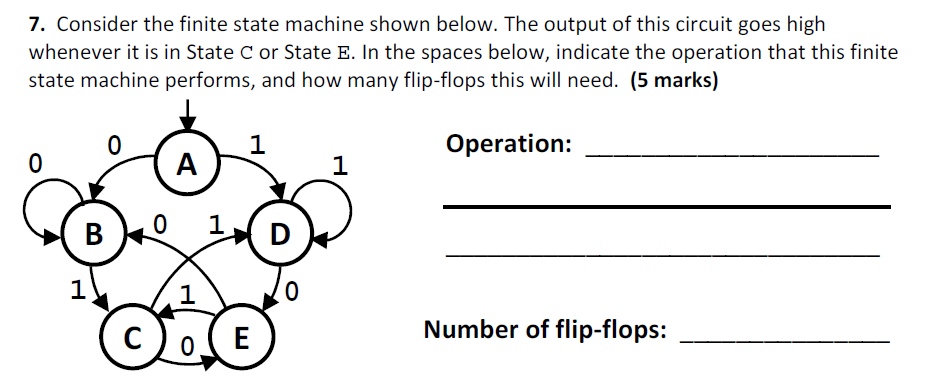
\includegraphics[width=0.9\textwidth]{FSM_1.png}
	\caption{example pic}
\end{figure}
\vspace{5mm}

Table Example
\begin{table}[htbp!]
	\centering
	\label{my-label}
	\begin{tabular}{lllllllll}
		& Bit7                      & Bit6                     & Bit5                             & Bit4                      & Bit3                     & Bit2                       & Bit1                      & Bit0                      \\ \cline{2-9} 
		\multicolumn{1}{l|}{00} & \multicolumn{1}{l|}{Wang} & \multicolumn{1}{l|}{Si}  & \multicolumn{1}{l|}{Tu}          & \multicolumn{1}{l|}{Shuo} & \multicolumn{1}{l|}{Wo}  & \multicolumn{1}{l|}{Cong}  & \multicolumn{1}{l|}{Wei}  & \multicolumn{1}{l|}{Jian} \\ \cline{2-9} 
		\multicolumn{1}{l|}{01} & \multicolumn{1}{l|}{Guo}  & \multicolumn{1}{l|}{You} & \multicolumn{1}{l|}{Ru}          & \multicolumn{1}{l|}{Ci}   & \multicolumn{1}{l|}{Hou} & \multicolumn{1}{l|}{Yan}   & \multicolumn{1}{l|}{Wu}   & \multicolumn{1}{l|}{Chi}  \\ \cline{2-9} 
		\multicolumn{1}{l|}{10} & \multicolumn{1}{l|}{Zhi}  & \multicolumn{1}{l|}{Tu}  & \multicolumn{1}{l|}{.}           & \multicolumn{1}{l|}{This} & \multicolumn{1}{l|}{is}  & \multicolumn{1}{l|}{Horse} & \multicolumn{1}{l|}{Fart} & \multicolumn{1}{l|}{,}    \\ \cline{2-9} 
		\multicolumn{1}{l|}{11} & \multicolumn{1}{l|}{I}    & \multicolumn{1}{l|}{am}  & \multicolumn{1}{l|}{Comfortable} & \multicolumn{1}{l|}{said} & \multicolumn{1}{l|}{by}  & \multicolumn{1}{l|}{Zhuge} & \multicolumn{1}{l|}{Cun}  & \multicolumn{1}{l|}{Fu}   \\ \cline{2-9} 
	\end{tabular}
	\caption{A pseudo $4\times 8$ bit Memory}
\end{table}

    
%    \newpage
%    
%    % bib stuff
%    \nocite{*}
%    \addtocontents{toc}{\protect\vspace{\beforebibskip}}
%    \addcontentsline{toc}{section}{\refname}    
%    \bibliographystyle{ieeetr}
 %   \bibliography{reference}
\end{document}